\begin{figure*}[t]
\centering
% ---------- build and measure the table ----------
\sbox{\kpnetbox}{%
\begin{minipage}[t]{0.48\textwidth}
\captionsetup{type=table}
\caption{Evaluation of annotation quality on KeypointNet \cite{you2020} correspondences.}
\label{tab:keypointnet_table}
\centering
\footnotesize
\setlength{\tabcolsep}{3.5pt}
\renewcommand{\arraystretch}{1.0}
\resizebox{\linewidth}{!}{%
\begin{tabular}{lcccc}
    \toprule
    Category & PCK@.05 $\uparrow$ & PCK@.10 $\uparrow$ & PCK@.15 $\uparrow$ & PCK@.20 $\uparrow$ \\
    \midrule
    Airplane   & 0.79 & 0.94 & 0.98 & 0.99 \\
    Bathtub    & 0.70 & 0.88 & 0.96 & 0.99 \\
    Bed        & 0.68 & 0.91 & 0.96 & 0.99 \\
    Bottle     & 0.83 & 0.96 & 0.98 & 0.99 \\
    Cap        & 0.80 & 0.97 & 1.0 & 1.00 \\
    Car        & 0.78 & 0.95 & 0.99 & 1.00 \\
    Chair      & 0.77 & 0.96 & 0.99 & 0.99 \\
    Guitar     & 0.81 & 0.96 & 0.98 & 0.99 \\
    Helmet     & 0.55 & 0.84 & 0.94 & 0.98 \\
    Knife      & 0.83 & 0.93 & 0.96 & 0.98 \\
    Laptop     & 0.89 & 0.99 & 1.00 & 1.00 \\
    Motorcycle & 0.75 & 0.93 & 0.98 & 0.99 \\
    Mug        & 0.73 & 0.96 & 0.99 & 1.00 \\
    Skateboard & 0.86 & 0.97 & 0.99 & 1.00 \\
    Table      & 0.76 & 0.96 & 0.99 & 1.00 \\
    Vessel     & 0.45 & 0.71 & 0.87 & 0.94 \\
    \midrule
    Mean       & 0.75 & 0.93 & 0.97 & 0.99 \\
    Median     & 0.78 & 0.96 & 0.98 & 0.99 \\
    \bottomrule
\end{tabular}%
}
\end{minipage}%
}
\setlength{\kpnetheight}{\dimexpr\ht\kpnetbox+\dp\kpnetbox\relax}
% 3 rows now; reserve ~3 baselines for the figure caption above the images.
\setlength{\kpimgheight}{\dimexpr(\kpnetheight - 3\baselineskip)/3\relax}
% ---------- left: table ----------
% ---------- right: 3 stacked images, full-width and full-height ----------
% \begin{minipage}[t][\kpnetheight][t]{0.48\textwidth}
% \captionof{figure}{Correspondences generated by our method on categories beyond existing datasets.}
% \label{fig:new_categories_examples}
% \centering
% 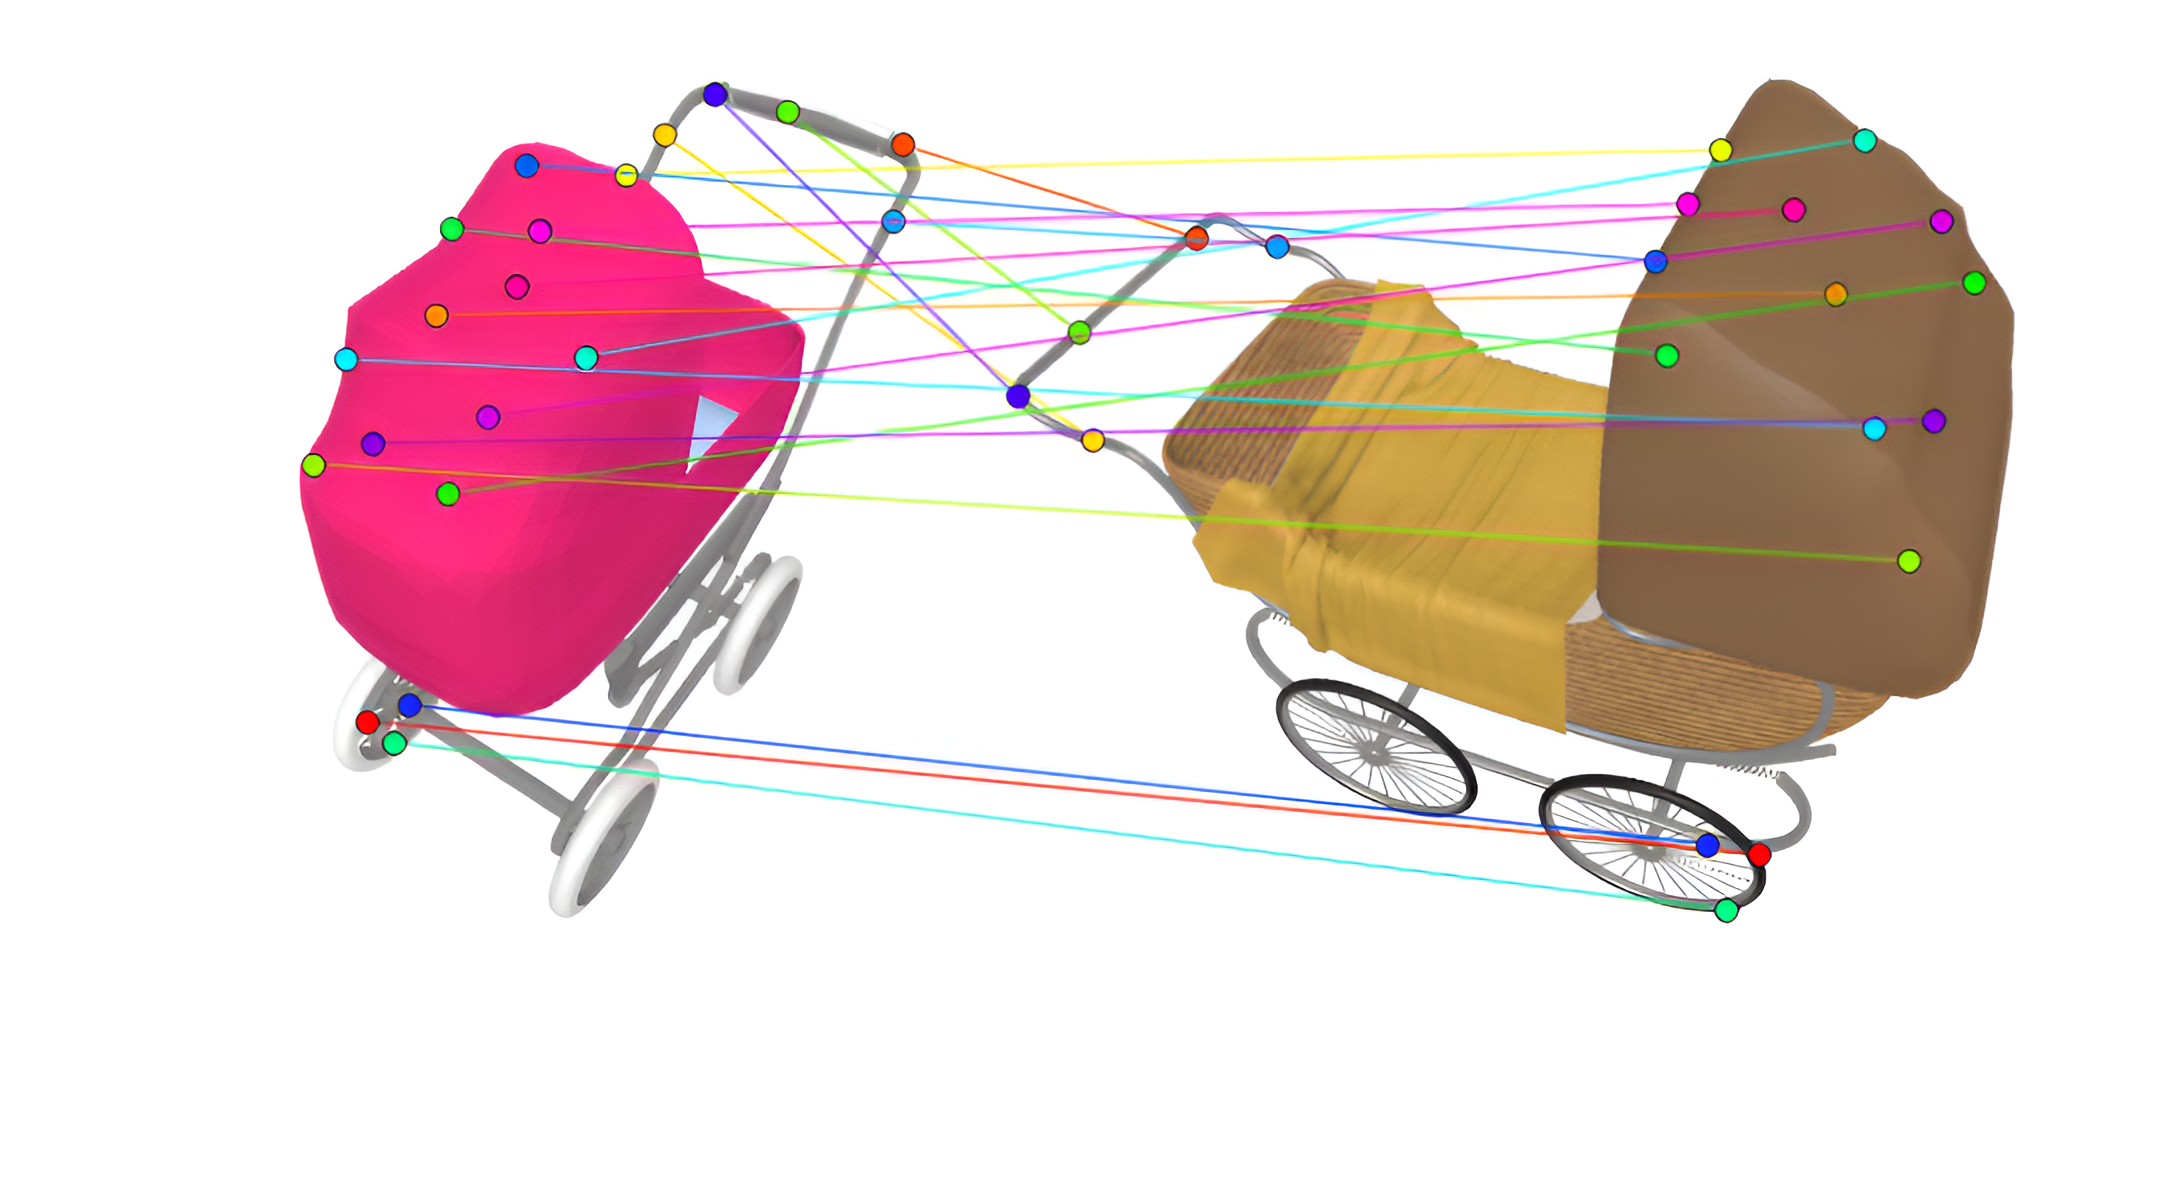
\includegraphics[width=\linewidth,height=\kpimgheight,trim={100 150 100 40},clip]{figures/matching_examples/baby_buggy_highres.png}\vfill
% 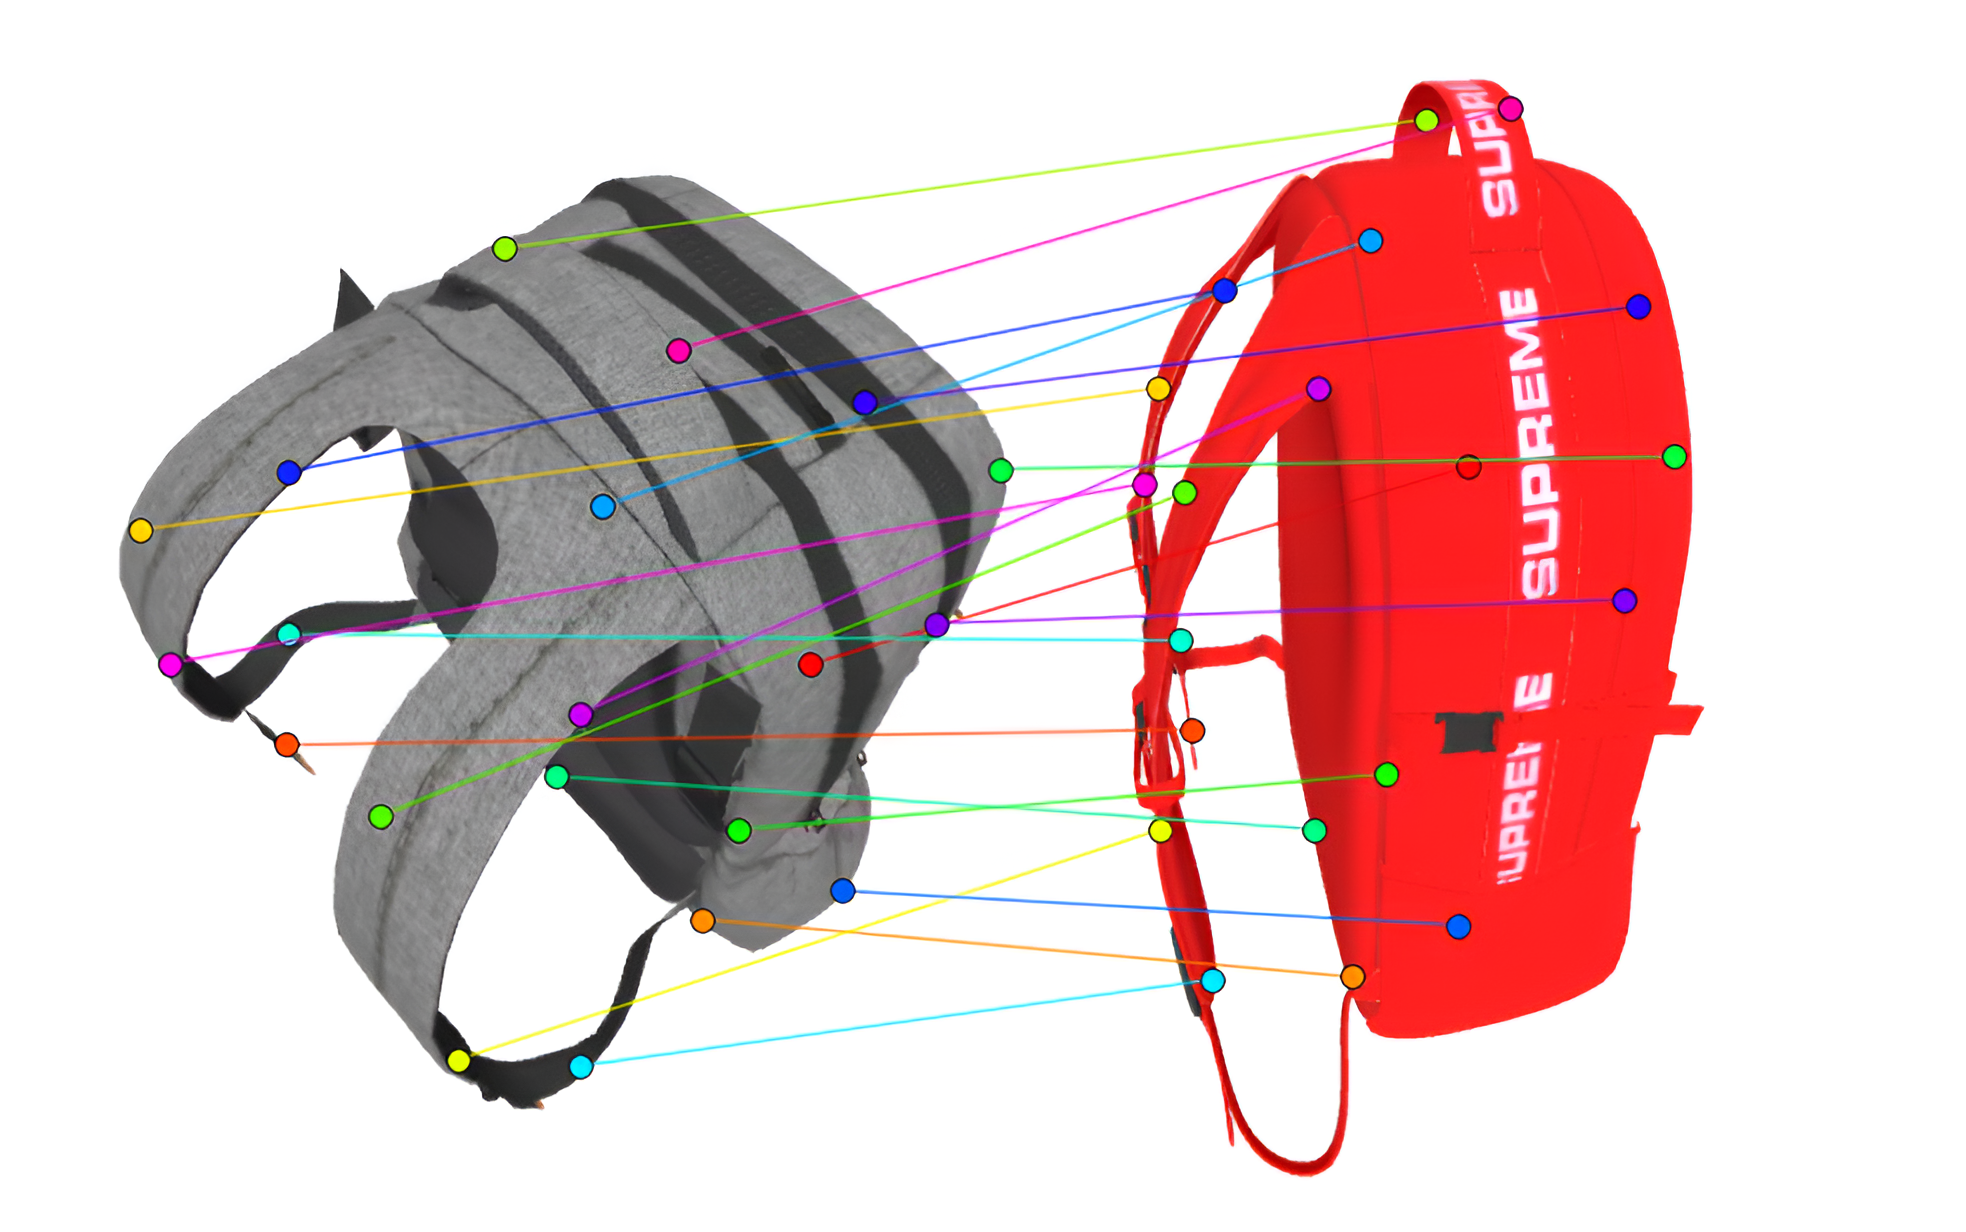
\includegraphics[width=\linewidth,height=\kpimgheight,trim={0 20 70 40},clip]{figures/matching_examples/backpack_highres.png}\vfill
% % 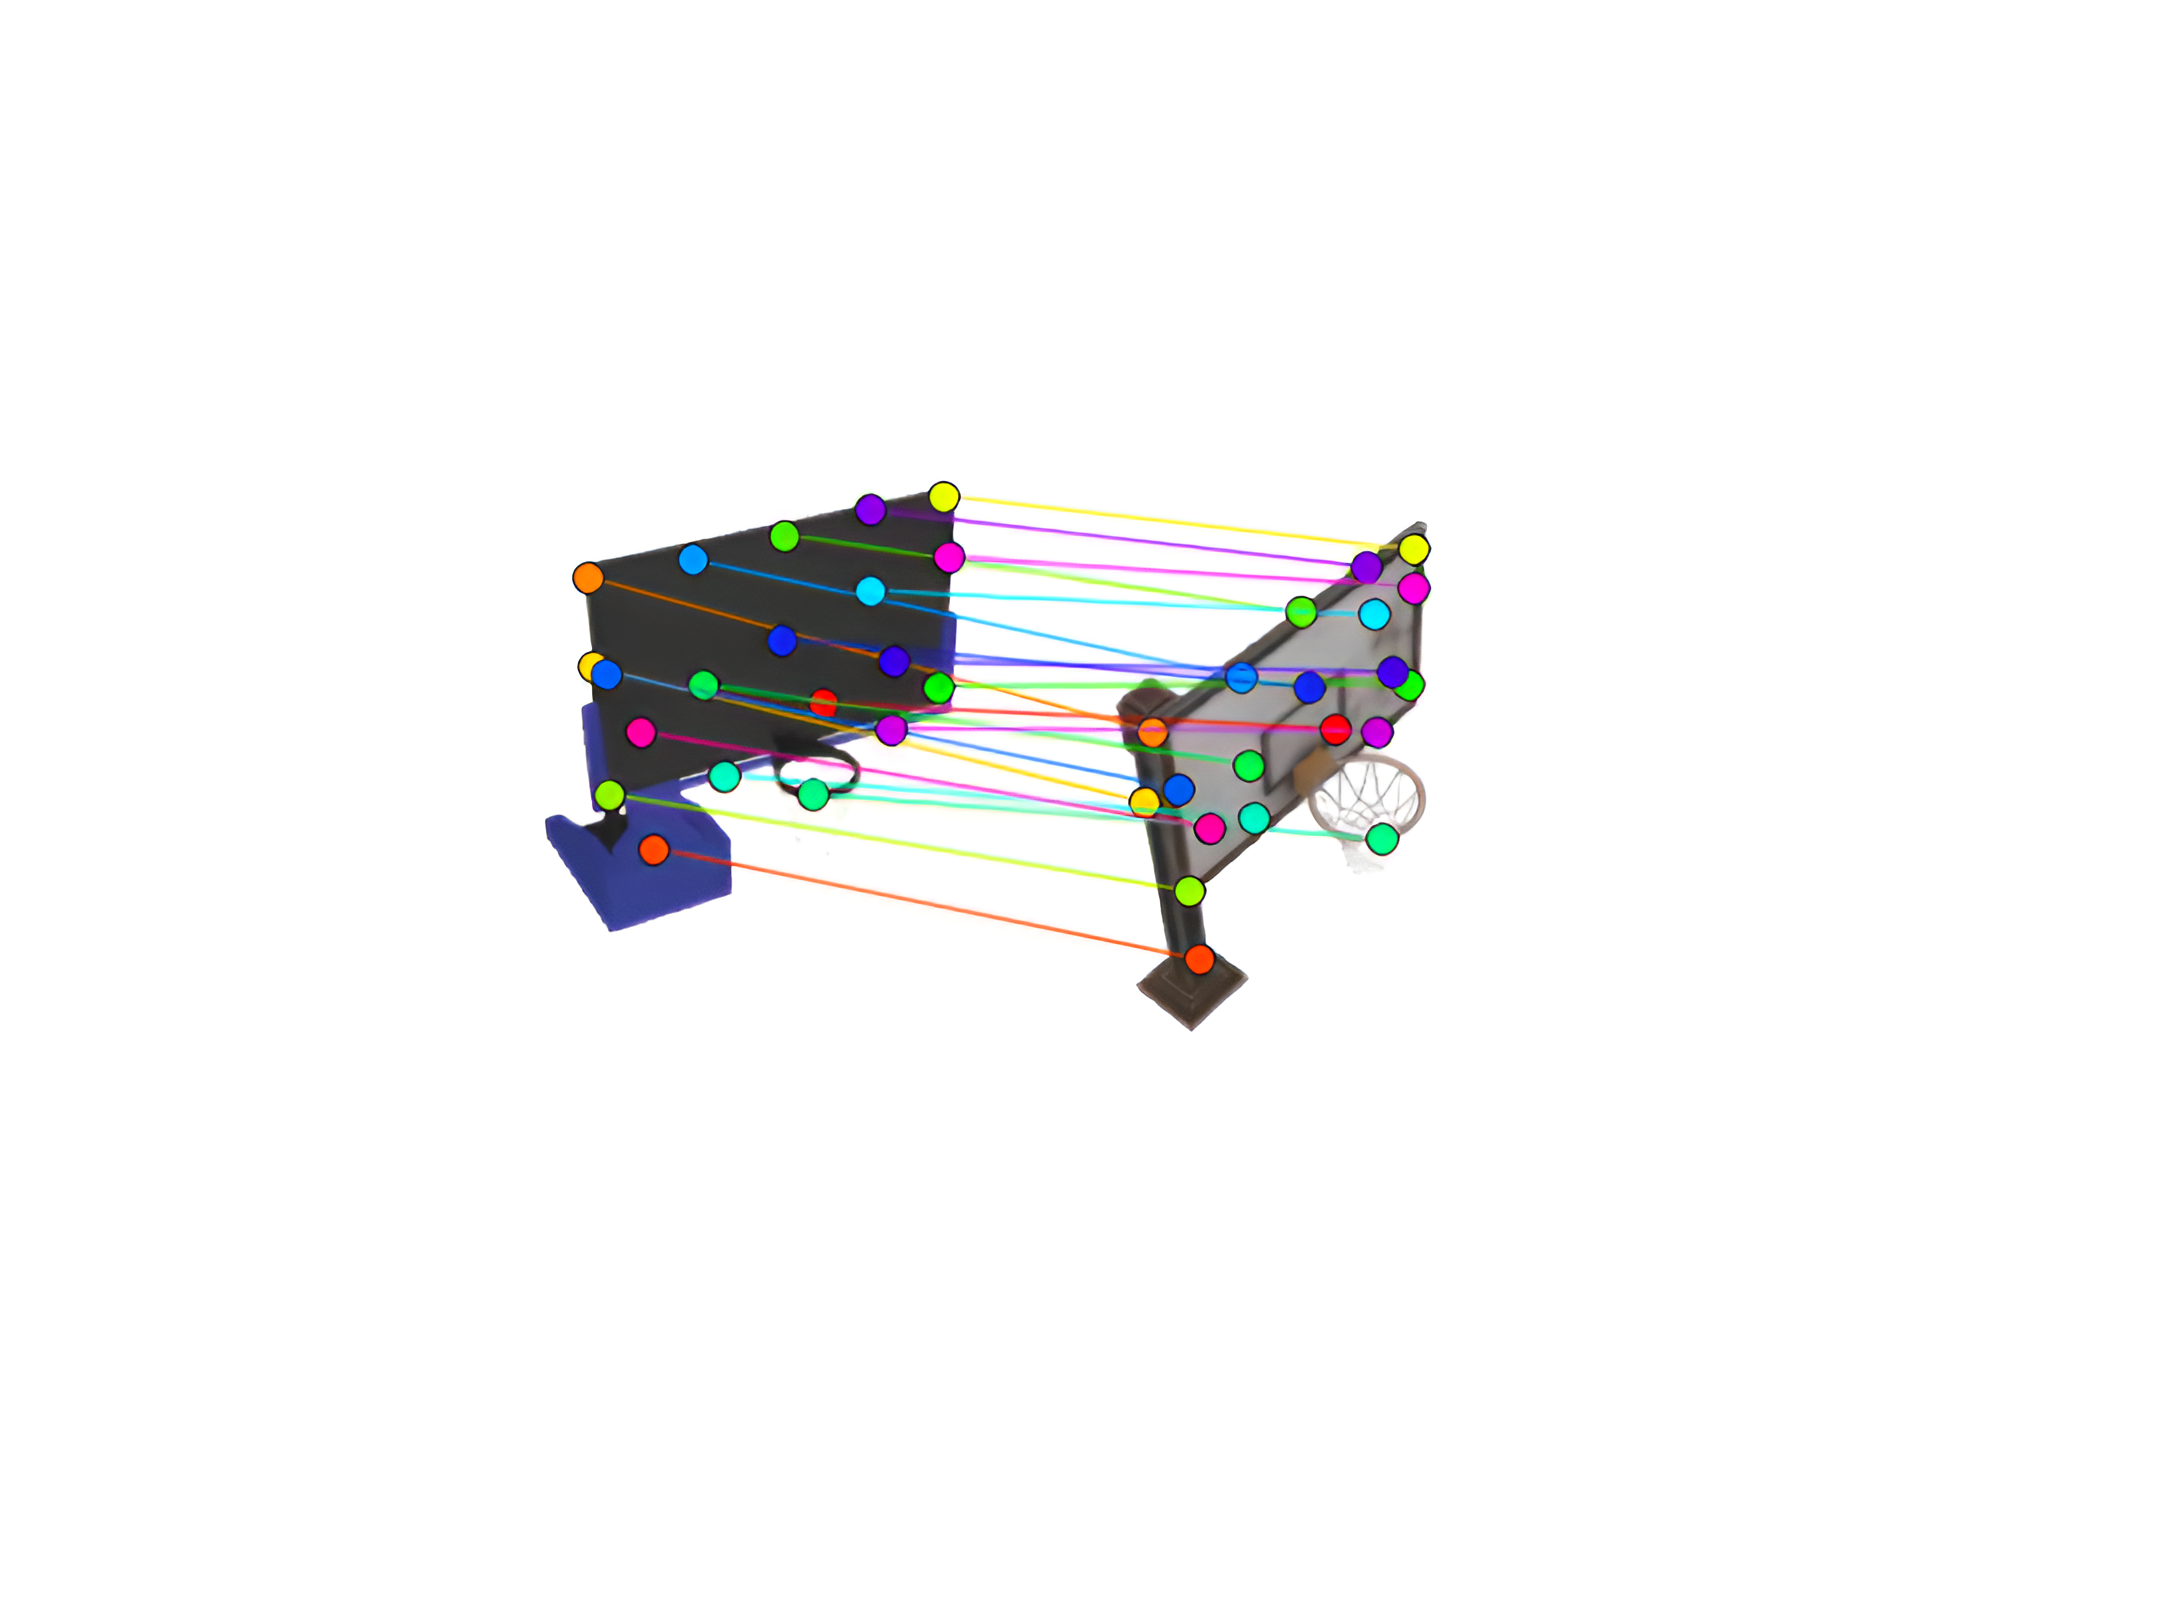
\includegraphics[width=\linewidth,height=\kpimgheight,trim={480 580 680 440},clip]{figures/matching_examples/basketball_higherres.png}
% 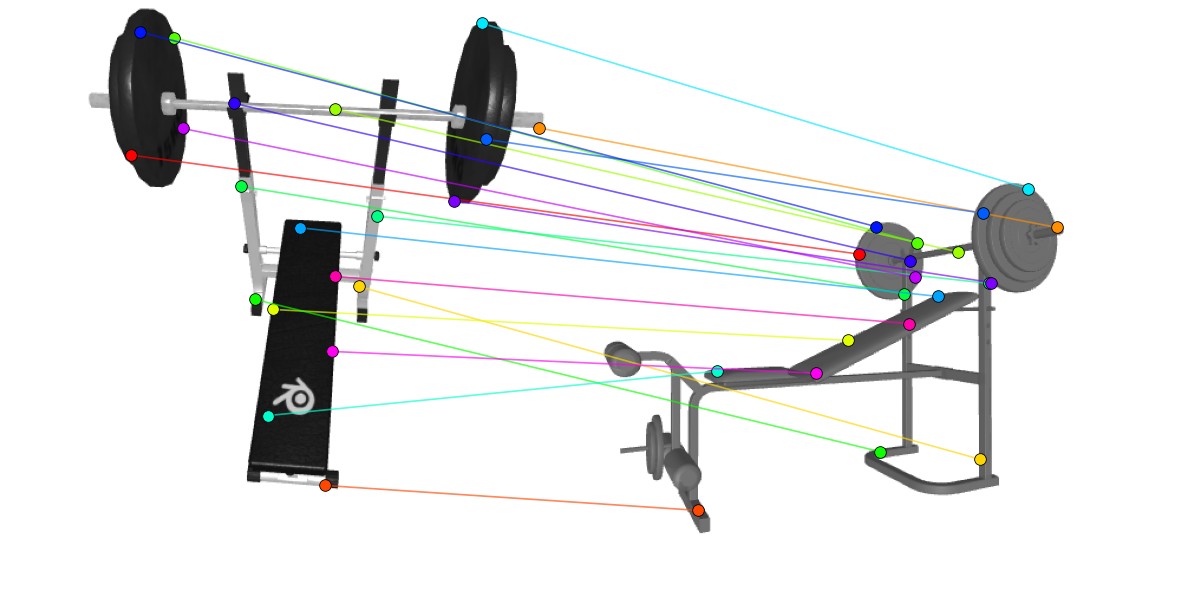
\includegraphics[width=\linewidth,height=\kpimgheight,trim={00 45 50 0},clip]{figures/matching_examples/barbell.png}
% \end{minipage}
% \end{figure*}

% ---------- left: table ----------
\makebox[\textwidth][c]{%
\usebox{\kpnetbox}%
\hfill%
%
\begin{minipage}[t][\kpnetheight][t]{0.504\textwidth}
\captionof{figure}{Qualitative SPair-71k results for MARCO \cite{cuttano2026marco}. Left: SPair71k-only. Right: ours-pretrained $\rightarrow$ SPair71k fine-tuned.}
\label{fig:qual_marco_main}
\centering
\scriptsize
\setlength{\tabcolsep}{0pt}

\begin{tabular}{cc}
\textbf{SPair-71k only} & \textbf{Ours P.T.$\rightarrow$SPair-71k} \\[0.2mm]

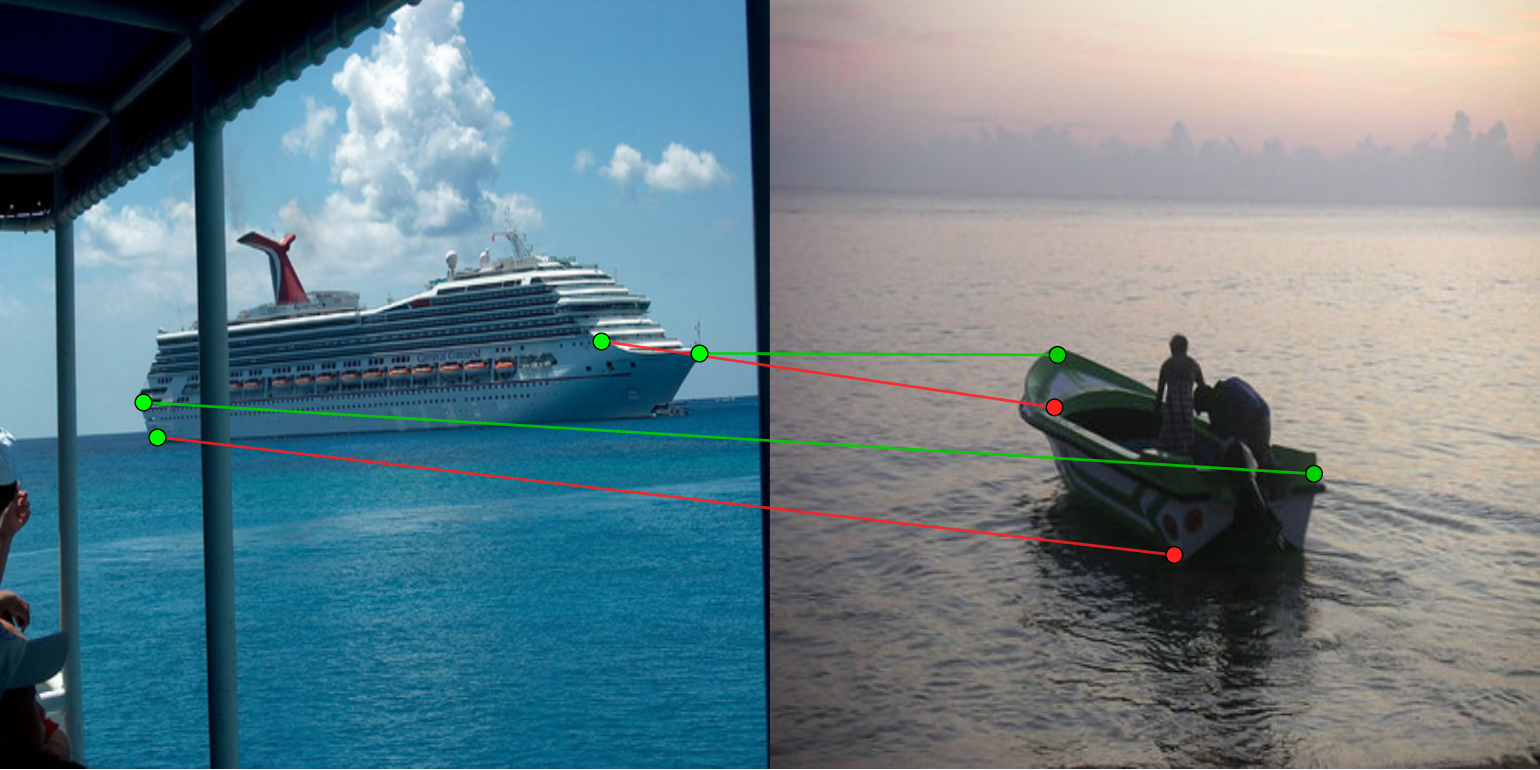
\includegraphics[width=0.49\linewidth]{figures/qualitative/marco/match_real_boat.png} &
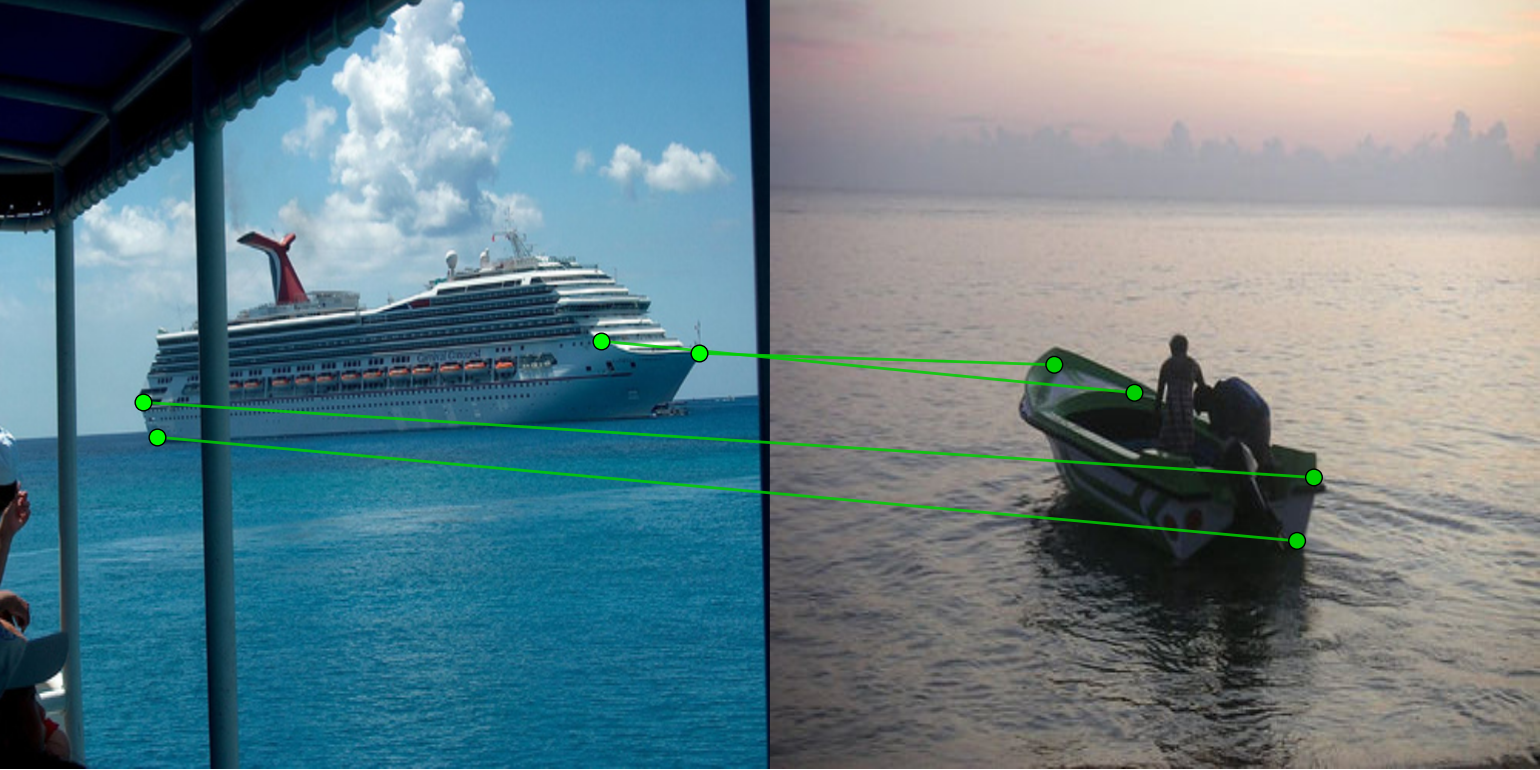
\includegraphics[width=0.49\linewidth]{figures/qualitative/marco/match_ours_boat.png} \\[-1mm]

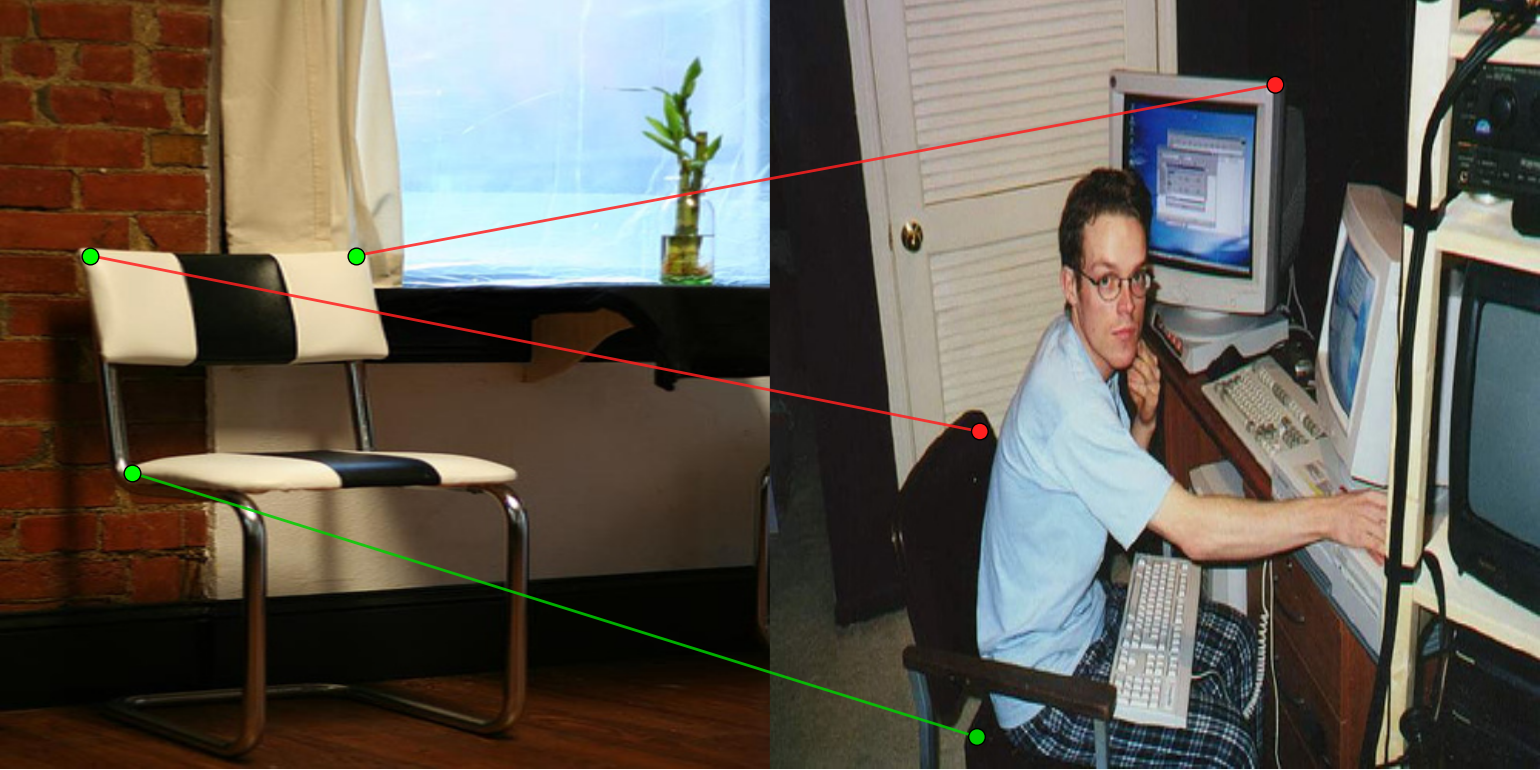
\includegraphics[width=0.49\linewidth]{figures/qualitative/marco/match_real_chair.png} &
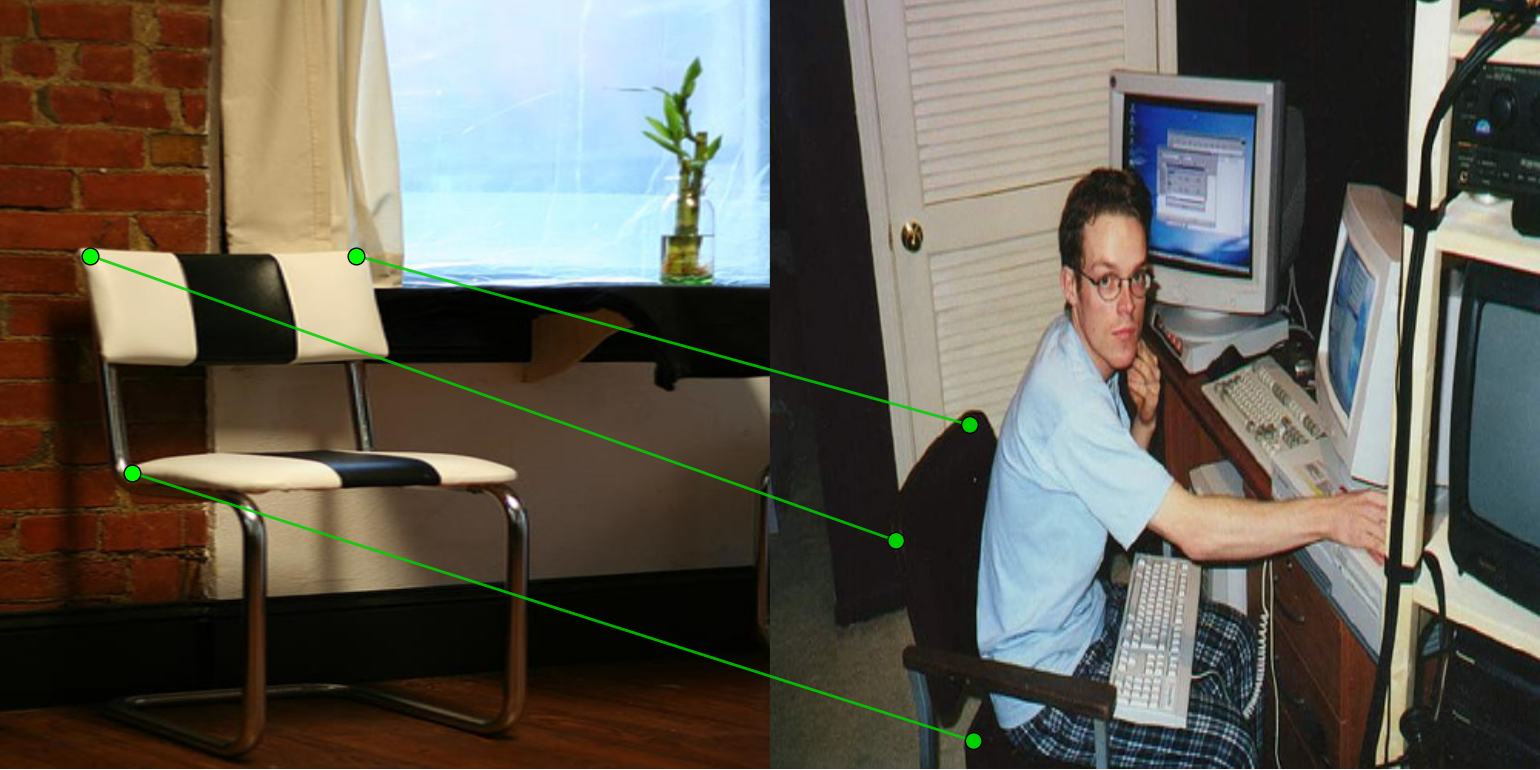
\includegraphics[width=0.49\linewidth]{figures/qualitative/marco/match_ours_chair.png}
 \\[-1mm]
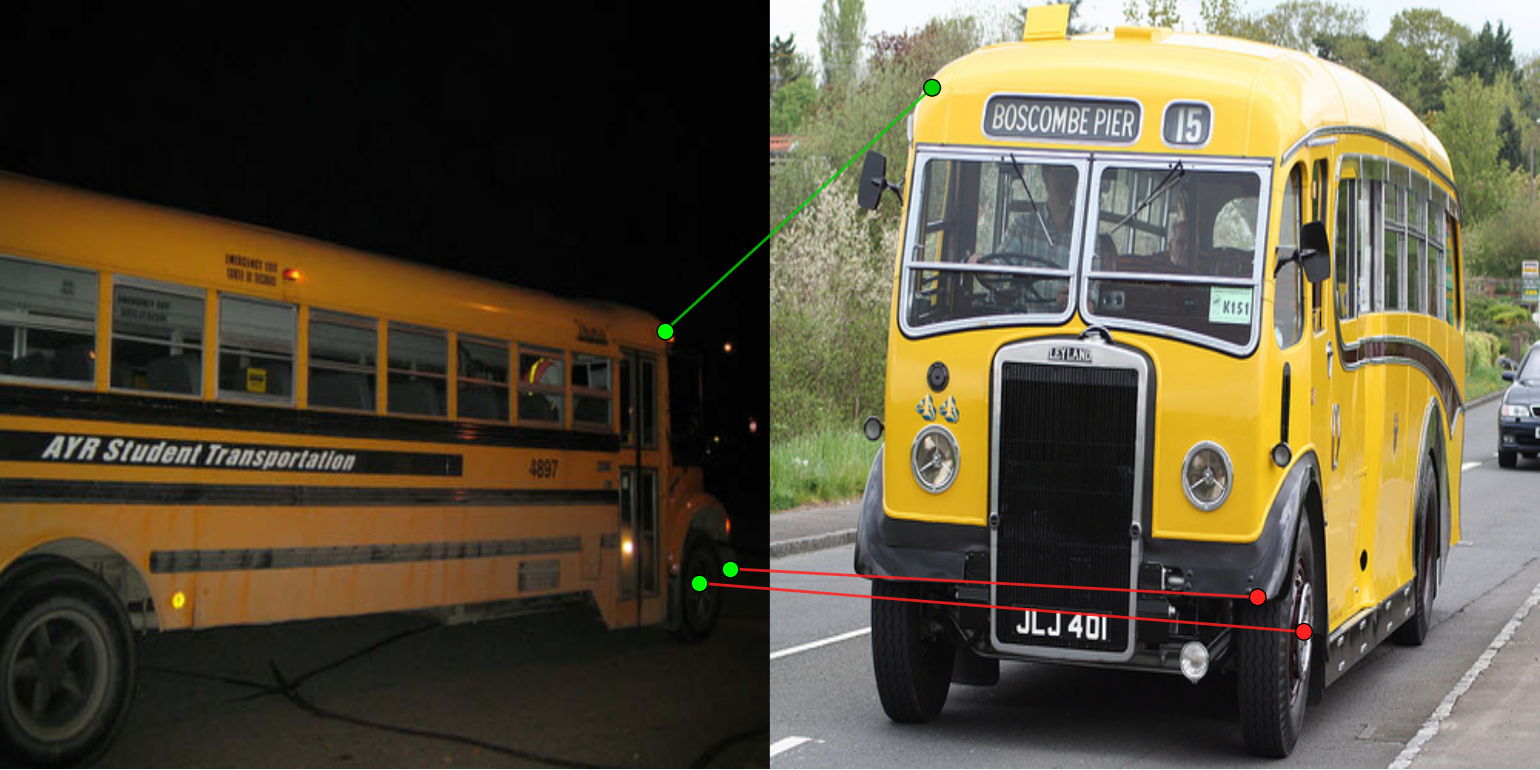
\includegraphics[width=0.49\linewidth]{figures/qualitative/marco/match_real_bus.png} &
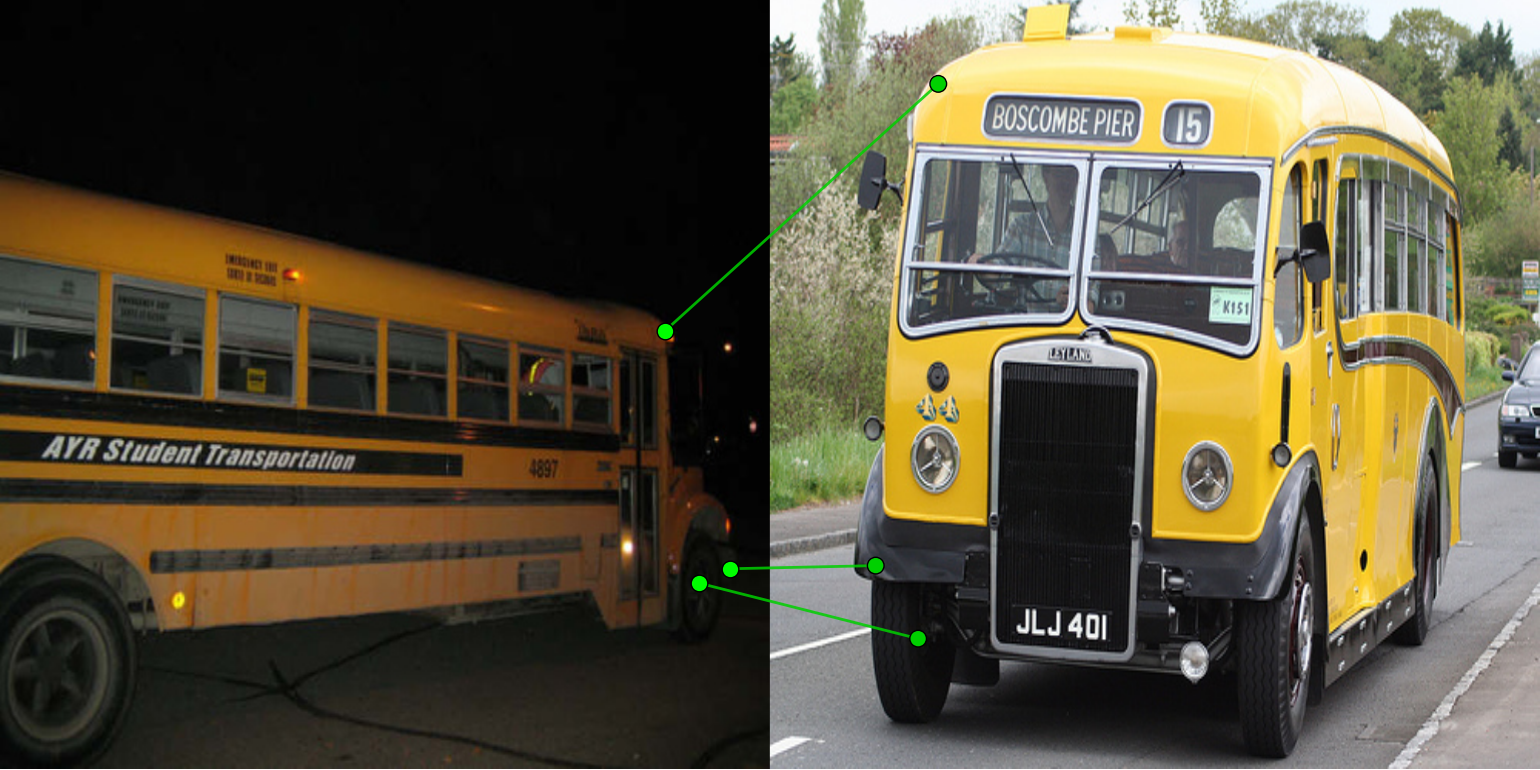
\includegraphics[width=0.49\linewidth]{figures/qualitative/marco/match_ours_bus.png}
\end{tabular}

\end{minipage}%
}
\end{figure*}




% \begin{table}[t]
%   \caption{Evaluation of annotation quality on KeypointNet correspondences.}
%   \label{tab:keypointnet_table}
%   \centering
%   \footnotesize
%   \setlength{\tabcolsep}{4pt}
%     \renewcommand{\arraystretch}{1.0}

%   \begin{tabular}{lcccc}
%     \toprule
%     Category & PCK@.05 $\uparrow$ & PCK@.10 $\uparrow$ & PCK@.15 $\uparrow$ & PCK@.20 $\uparrow$ \\
%     \midrule
%     Airplane   & 0.79 & 0.94 & 0.98 & 0.99 \\
%     Bathtub    & 0.70 & 0.88 & 0.96 & 0.99 \\
%     Bed        & 0.68 & 0.91 & 0.96 & 0.99 \\
%     Bottle     & 0.83 & 0.96 & 0.98 & 0.99 \\
%     Cap        & 0.76 & 0.94 & 0.99 & 1.00 \\
%     Car        & 0.78 & 0.95 & 0.99 & 1.00 \\
%     Chair      & 0.77 & 0.96 & 0.99 & 0.99 \\
%     Guitar     & 0.81 & 0.96 & 0.98 & 0.99 \\
%     Helmet     & 0.41 & 0.75 & 0.90 & 0.96 \\
%     Laptop     & 0.89 & 1.00 & 1.00 & 1.00 \\
%     Motorcycle & 0.75 & 0.93 & 0.98 & 0.99 \\
%     Mug        & 0.73 & 0.96 & 0.99 & 1.00 \\
%     Skateboard & 0.86 & 0.97 & 0.99 & 1.00 \\
%     Table      & 0.76 & 0.96 & 0.99 & 1.00 \\
%     Vessel     & 0.45 & 0.72 & 0.87 & 0.94 \\
%     Knife      & 0.83 & 0.93 & 0.96 & 0.98 \\
%     \midrule
%     Mean       & 0.74 & 0.92 & 0.97 & 0.99 \\
%     Median     & 0.76 & 0.95 & 0.98 & 0.99 \\
%     \bottomrule
%   \end{tabular}
% \end{table}



\begin{comment}
\captionsetup{type=table}
\caption{Evaluation of annotation quality on KeypointNet \cite{you2020} correspondences.}
\label{tab:keypointnet_table}
\centering
\footnotesize
\setlength{\tabcolsep}{3.5pt}
\renewcommand{\arraystretch}{1.0}
\resizebox{\linewidth}{!}{%
\begin{tabular}{lcccc}
    \toprule
    Category & PCK@.05 $\uparrow$ & PCK@.10 $\uparrow$ & PCK@.15 $\uparrow$ & PCK@.20 $\uparrow$ \\
    \midrule
    Airplane   & 0.79 & 0.94 & 0.98 & 0.99 \\
    Bathtub    & 0.70 & 0.88 & 0.96 & 0.99 \\
    Bed        & 0.68 & 0.91 & 0.96 & 0.99 \\
    Bottle     & 0.83 & 0.96 & 0.98 & 0.99 \\
    Cap        & 0.76 & 0.94 & 0.99 & 1.00 \\
    Car        & 0.78 & 0.95 & 0.99 & 1.00 \\
    Chair      & 0.77 & 0.96 & 0.99 & 0.99 \\
    Guitar     & 0.81 & 0.96 & 0.98 & 0.99 \\
    Helmet     & 0.41 & 0.75 & 0.90 & 0.96 \\
    Laptop     & 0.89 & 1.00 & 1.00 & 1.00 \\
    Motorcycle & 0.75 & 0.93 & 0.98 & 0.99 \\
    Mug        & 0.73 & 0.96 & 0.99 & 1.00 \\
    Skateboard & 0.86 & 0.97 & 0.99 & 1.00 \\
    Table      & 0.76 & 0.96 & 0.99 & 1.00 \\
    Vessel     & 0.45 & 0.72 & 0.87 & 0.94 \\
    Knife      & 0.83 & 0.93 & 0.96 & 0.98 \\
    \midrule
    Mean       & 0.74 & 0.92 & 0.97 & 0.99 \\
    Median     & 0.76 & 0.95 & 0.98 & 0.99 \\
    \bottomrule
\end{tabular}%
}
\end{comment}